\section{Exact Energy-Guided Sampling}
To perform energy-guided sampling for \eqref{Eq:target_distribution_intro}, the guidance during the sampling procedure needs to guarantee that final samples follow the desired distribution $p(\x)$.
In this section, we propose an exact formulation of such energy guidance and propose a novel training objective to estimate the guidance. All the proofs can be found in Appendix~\ref{appendix:proof}.









\subsection{Exact Formulation of Intermediate Energy Guidance}
\label{Sec:problem}
	
	

\begin{figure}[t]
    \begin{minipage}{0.14\linewidth}
        \centering 
        \scriptsize{$q_t(\x_t)$}
    \end{minipage}
    \begin{minipage}{0.85\linewidth}
		\centering
		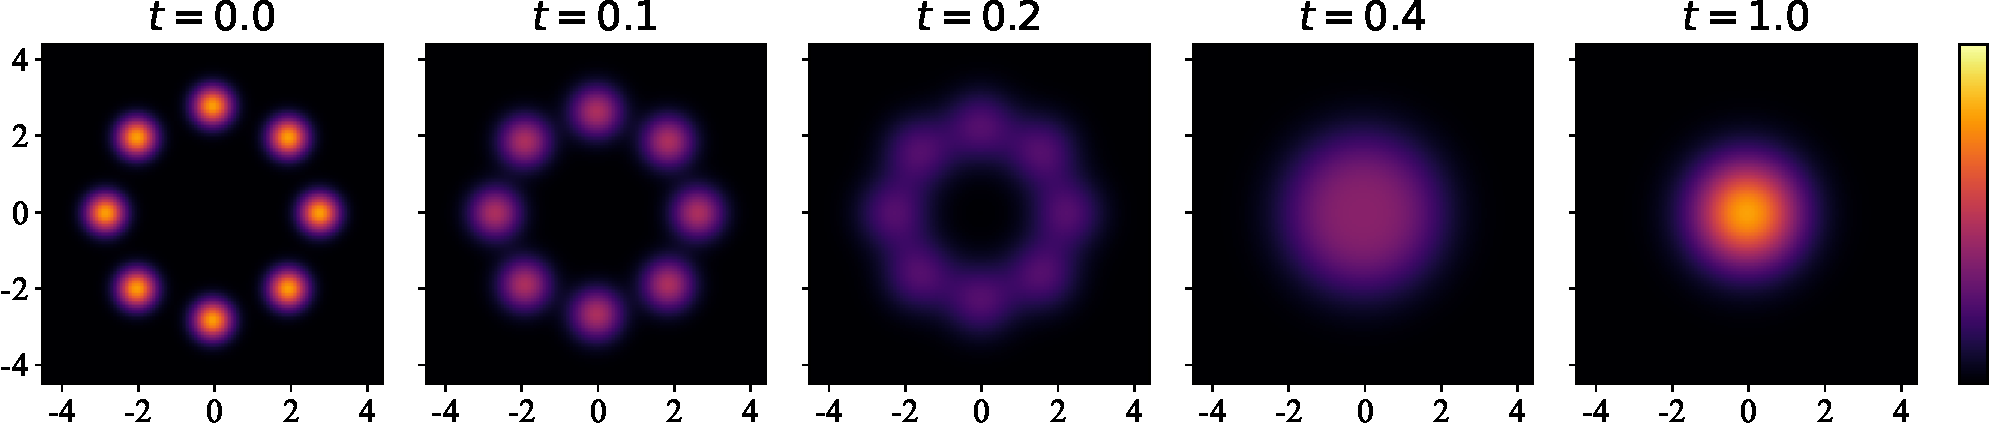
\includegraphics[width=\linewidth]{pics/toy_energy/mu_t-crop.pdf}
	\end{minipage} \\
	
	\begin{minipage}{0.14\linewidth}
        \centering 
        \scriptsize{$e^{-\gE_t(\x_t)}$}
    \end{minipage}
    \begin{minipage}{0.85\linewidth}
		\centering
		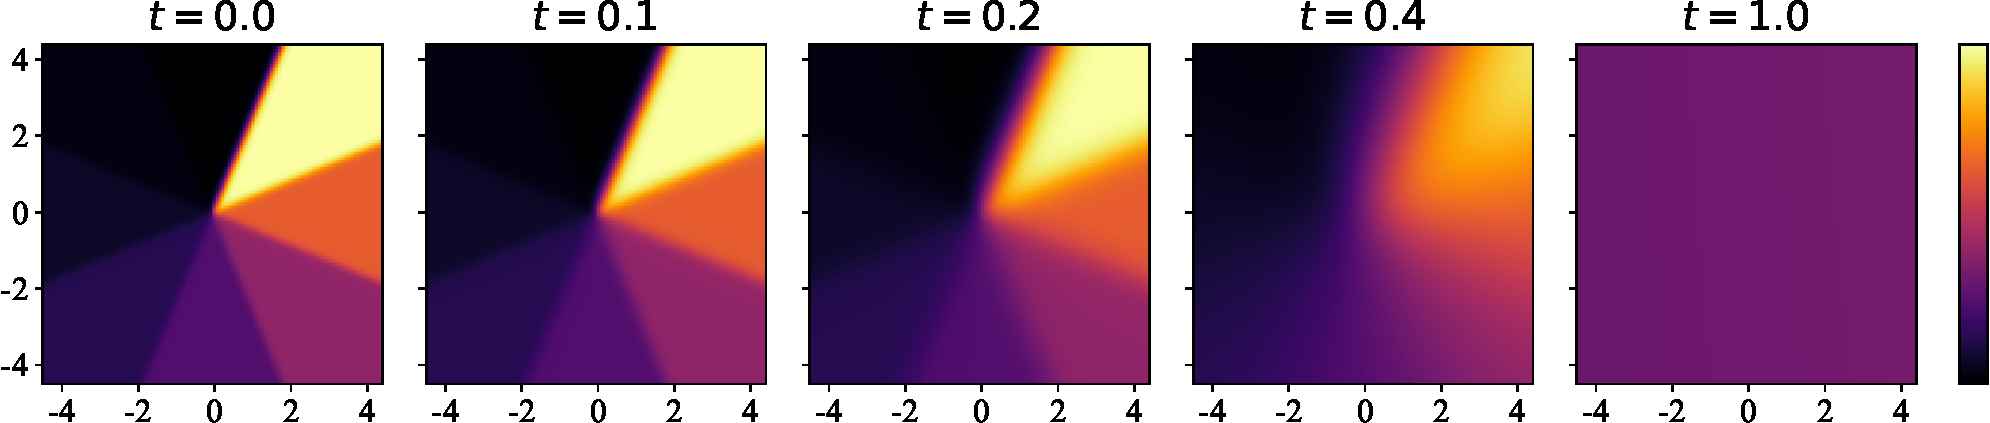
\includegraphics[width=\linewidth]{pics/toy_energy/expq_t-crop.pdf}
	\end{minipage} \\
	
	\begin{minipage}{0.14\linewidth}
        \centering 
        \scriptsize{$p_t(\x_t)$}
    \end{minipage}
    \begin{minipage}{0.85\linewidth}
		\centering
		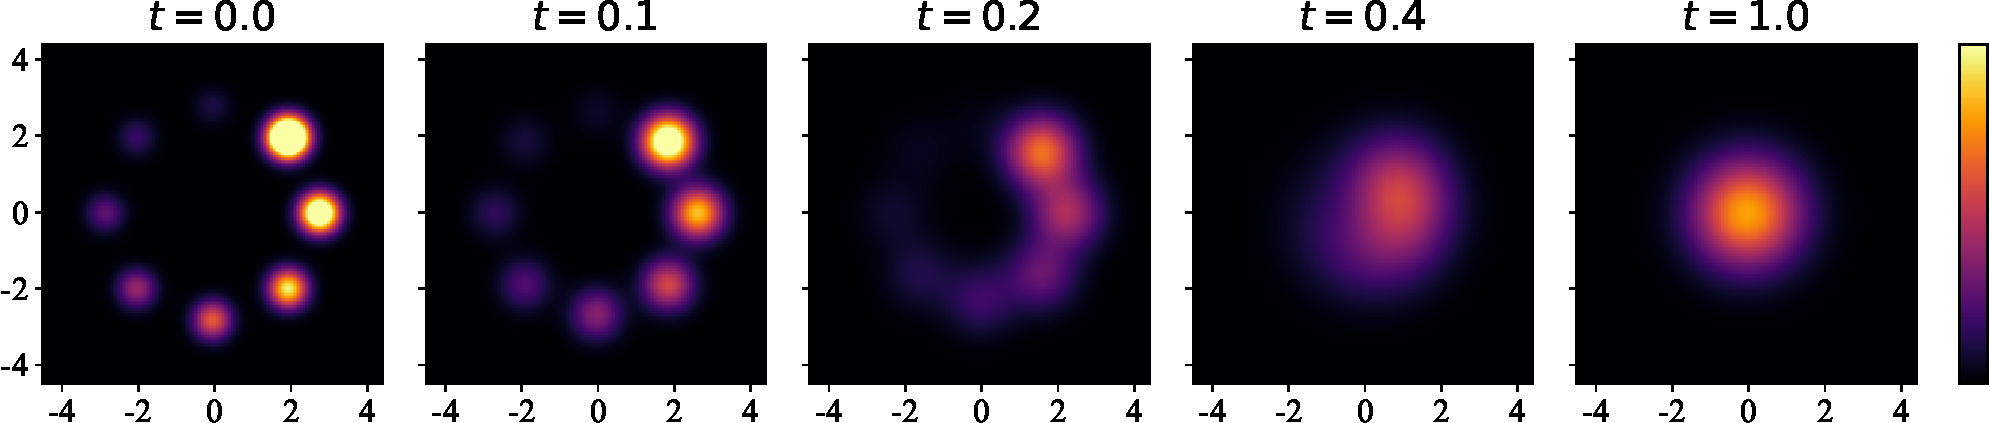
\includegraphics[width=\linewidth]{pics/toy_energy/mix_t-crop.pdf}
	\end{minipage}
	\vspace{-0.05in}
	\caption{\label{fig:intermediate_energy}\small{A 2-D mixtures-of-Gaussians example of the density functions (unnormalized) for $q_t(\x_t)$, $e^{-\gE_t(\x_t)}$ and $p_t(\x_t)$ during the diffusion process, where $p_t(\x_t)\propto q_t(\x_t)e^{-\gE_t(\x_t)}$.}}
	\vspace{-0.15in}
\end{figure}


Below we formally analyze how to sample from \eqref{Eq:target_distribution_intro} by diffusion models.

Rewrite $p_0 \coloneqq p$ and $q_0\coloneqq q$. The target distribution is
\begin{equation}
\label{Eq:target_distribution}
    p_0(\x_0) \propto q_0(\x_0)e^{-\beta\gE(\x_0)}.
\end{equation}
Let $q_t(\x_t)$ be the marginal distribution of the forward diffusion process at time $t$ defined in \eqref{Eq:forward_diffusion} starting from $q_0(\x_0)$. 
Suppose we have a pretrained diffusion model $q^{\theta}_0(\x_0)\approx q_0(\x_0)$ by learning a noise prediction model $\epsilonv_\theta(\x_t,t)\approx -\sigma_t\nabla_{\x_t}\log q_t(\x_t)$ parameterized by $\theta$ at each time $t\in[0,T]$. By \eqref{Eq:diffusion_ode}, drawing samples from $p_0$ requires the corresponding score functions $\nabla_{\x_t}\log p_t(\x_t)$ at each intermediate time $t$ of the diffusion process starting from $p_0$ instead of $q_0$. 
Our first key result is on revealing the relationship between the corresponding score functions during the diffusion processes starting from $q_0$ and $p_0$, as summarized below:




\begin{theorem}[Intermediate Energy Guidance]
\label{thrm:intermediate_energy_guidance}
Suppose $q_0$ and $p_0$ are defined as in \eqref{Eq:target_distribution}. For $t\in(0, T]$, let
\begin{equation}
\label{Eq:forward_p}
    p_{t0}(\x_t|\x_0) \coloneqq q_{t0}(\x_t|\x_0) = \gN(\x_t|\alpha_t\x_0,\sigma_t^2\mI).
\end{equation}
Denote $q_t(\x_t):=\int q_{t0}(\x_t|\x_0) q_0(\x_0)\dm\x_0$ and $p_t(\x_t):=\int p_{t0}(\x_t|\x_0) p_0(\x_0)\dm\x_0$ as the marginal distributions at time $t$, and define
\begin{equation}
\label{Eq:intermediate_energy}
    \gE_t(\x_t)\! \coloneqq\! \left\{
    \begin{array}{ll}
        \beta\gE(\x_0), & t=0, \\
        -\log \E_{q_{0t}(\x_0|\x_t)}\left[
        e^{-\beta\gE(\x_0)}
        \right], & t > 0.
    \end{array} \right.
\end{equation}
Then $q_t$ and $p_t$ satisfy
\begin{equation}
    \label{Eq:pt_qt_Et}
    p_t(\x_t) \propto q_t(\x_t)e^{-\gE_t(\x_t)},
\end{equation}
and their score functions satisfy
\begin{equation}
\label{Eq:energy_guidance}
    \nabla_{\x_t}\log p_t(\x_t) = \underbrace{\nabla_{\x_t}\log q_t(\x_t)}_{\approx -\epsilonv_\theta(\x_t,t)/\sigma_t}
    - \underbrace{\nabla_{\x_t}\gE_t(\x_t)}_{\substack{\text{energy guidance}\\\text{\color{red}{\textbf{(intractable)}}}}}.
\end{equation}
\vspace{-0.2in}
\end{theorem}






\cref{thrm:infoNCE_energy} reveals a previously unnoticed exact form of the intermediate distributions $p_t$: though $p_t$ is defined as an intractable marginal distribution for all $t>0$, they could still be written \emph{in the same form} as  Eq.~(\ref{Eq:target_distribution}), proportional to the product of the (diffused) data distribution $q_t$ and an exponential energy term $e^{-\gE_t(\x_t)}$.
Since such energy is defined during the diffusion process, we name $\gE_t(\cdot)$ as \textit{intermediate energy}.
According to \eqref{Eq:intermediate_energy}, the intermediate energy is completely determined by the energy function $\gE(\x_0)$ at time $0$.
An illustration is given in \cref{fig:intermediate_energy}, from which we draw several observations: (1) $p_t(\x_t)$ prefers areas with both high data density $q_t(\x_t)$ and high energy density $e^{-\gE_t(\x_t)}$; (2) Through the forward diffusion process, both $p_t$ and $q_t$ gradually become standard Gaussian, which guarantees that we can reverse the diffusion process starting from the same noise distribution $p_T \approx q_T \approx \gN(0, \tilde\sigma^2\mI)$; (3) The energy function $\gE_0(\x_0)$ is also ``diffused'' into intermediate energy functions $\gE_t(\x_t)$ as $t$ increases. In particular, $\gE_T(\x_T)$ is almost equal to a constant function and thus $\nabla_{\x_T}\gE_T(\x_T) \approx 0$.
 

The result in \eqref{Eq:energy_guidance} directly defines a principled method to perform guided sampling from $p_0(\x_0)$. 
Namely, we can sample with \eqref{Eq:diffusion_ode} as along as we know both $\nabla_{\x_t}\log q_t(\x_t)$ and $\nabla_{\x_t}\gE_t(\x_t)$.
The former score is already given by the pretrained diffusion model $\epsilonv_\theta$. 
The remaining problem is to estimate the latter score $\nabla_{\x_t}\gE_t(\x_t)$, which we name as \emph{intermediate energy guidance}.
An unbiased estimation of $\nabla_{\x_t}\gE_t(\x_t)$ is generally non-trivial due to the log-expectation formulation and a potentially complex form of $\gE(\x_0)$ in \eqref{Eq:intermediate_energy}. To the best of our knowledge, it is still an open problem for estimating the exact intermediate energy guidance. 
We present a first attempt by developing a novel learning-based method to learn the energy guidance by comparing energy of samples from $q_t$, as detailed below.
















\subsection{Learning Energy Guidance by Contrastive Energy Prediction}
\label{Sec:method}




Let $K>1$ be a positive integer. Let $\x_0^{(1)},\dots,\x_0^{(K)}$ be $K$ i.i.d. samples from $q_0(\x_0)$ and $\epsilonv^{(1)},\dots,\epsilonv^{(K)}$ be $K$ i.i.d. Gaussian samples following $p(\epsilonv)=\gN(\epsilonv|\bm{0}, \mI)$. Let $t \sim \mathcal{U}(0,T)$ be a randomly sampled time step. For each $i=1,\dots,K$, let $\x_t^{(i)}\coloneqq \alpha_t\x_0^{(i)} + \sigma_t\epsilonv^{(i)}$, where $\alpha_t,\sigma_t$ are defined in \eqref{Eq:forward_p}. Assume that the intermediate energy $\gE_t(\cdot)$ is approximated by a network $f_\phi(\cdot,t):\R^d\rightarrow \R$ parameterized by $\phi$. We propose to solve the following problem to learn $f_\phi$, whose solution is characterized in \cref{thrm:infoNCE_energy}:
\begin{equation}
\label{Eq:infoNCE_energy}
\begin{split}
    &\min_\phi \E_{p(t)}\E_{q_0(\x_0^{(1:K)})}\E_{p(\epsilonv^{(1:K)})}\Bigg[ \\
    &- \sum_{i=1}^K
    \underbrace{%
        \vphantom{\frac{\exp(-f_\phi(\x_t^{(i)},t))}{\sum_{j=1}^K \exp(-f_\phi(\x_t^{(j)},t))}} 
         e^{-\beta\gE(\x_0^{(i)})}
    }_{\text{soft energy label}}
    \log \underbrace{\frac{e^{-f_\phi(\x_t^{(i)},t)}}{\sum_{j=1}^K e^{-f_\phi(\x_t^{(j)},t)}}}_{\text{predicted label}}
\Bigg].
 \end{split}
\end{equation}
\begin{theorem}
\label{thrm:infoNCE_energy}

Given unlimited model capacity and data samples, For all $K>1$ and $t\in[0,T]$, the optimal $f_{\phi^*}$ in problem (\ref{Eq:infoNCE_energy}) satisfies $\nabla_{\x_t}f_{\phi^*}(\x_t,t) = \nabla_{\x_t}\gE_t(\x_t)$.
\end{theorem}

According to \cref{thrm:infoNCE_energy}, we indeed can train the energy guidance model $f_\phi$ by solving problem (\ref{Eq:infoNCE_energy}) and use the gradients of $f_\phi$ for guided sampling by estimating the energy guidance in \eqref{Eq:energy_guidance}.
Here we give an intuitive explanation of \cref{thrm:infoNCE_energy}. To estimate the energy guidance $\nabla_{\x_t}\gE_t(\cdot)$, we only need to ensure $f_\phi$ to be a relative proportional value of $\gE_t(\cdot)$, so it is enough to relatively compare $f_\phi$ within $K$ samples instead of directly train $f_\phi$ with the absolute values. Built upon such an observation, we leverage a cross-entropy loss in problem (\ref{Eq:infoNCE_energy}), where the energy $\gE(\x_0^{(i)})$ of $K$ clean samples $\x_0^{(i)}$ are soft supervising labels and the softmax of energy predictions $f_\phi(\x_t^{(i)},t)$ of $K$ noisy samples $\x_t^{(i)}$ are predicted labels.
Due to the contrastive manner of this objective, we name our proposed method in \eqref{Eq:infoNCE_energy} as \textit{Contrastive Energy Prediction (CEP)}.






Although the optimal solution in problem (\ref{Eq:infoNCE_energy}) is exact, sometimes we may suffer from numerical issues during training because the exponential term $e^{-\beta\gE(\x_0^{(i)})}$ is unnormalized. For example, suppose $\gE(\x_0)$ is a complex function that might contain ``spikes'' at some data point, the exponential term will greatly amplify such instability during training. To address this issue, we further use a self-normalized energy label by normalizing the energy function across the $K$ samples and define the optimization problem as:
\begin{equation}
\label{Eq:infoNCE_energy_normalized}
\begin{split}
    &\min_\phi \E_{p(t)}\E_{q_0(\x_0^{(1:K)})}\E_{p(\epsilonv^{(1:K)})}\Bigg[ \\
    &- \sum_{i=1}^K \!
    \underbrace{\frac{e^{-\beta\gE(\x_0^{(i)})}}{\sum_{j=1}^K e^{-\beta\gE(\x_0^{(j)})}}}_{\text{self-normalized energy label}}
    \log \underbrace{\frac{e^{-f_\phi(\x_t^{(i)},t)}}{\sum_{j=1}^K e^{-f_\phi(\x_t^{(j)},t)}}}_{\text{predicted label}}
\Bigg].
\end{split}
\end{equation}
Such a self-normalized objective can ensure the soft energy label is within $[0,1]$ and the sum of each item is exactly $1$. Although this objective may be biased against the original one in problem (\ref{Eq:infoNCE_energy}), we empirically find that it can greatly improve the numerical stability and help to achieve a good converged result. Moreover, we can reduce bias in the objective by increasing $K$. For $K\rightarrow \infty$, the objective in (\ref{Eq:infoNCE_energy_normalized}) is equivalent to that in (\ref{Eq:infoNCE_energy}) because $\sum_{\x_0}  e^{-\beta\gE(\x_0)} = \E_{q_0(\x_0)}[e^{-\beta\gE(\x_0)}]$ is the normalizing constant of $p_0$. Therefore, a larger $K$ is preferred in practice given enough computation and memory budget.










